\chapter{Opis użytych algorytmów}
Projekt został wyposażony w trzy algorytmy wyszukujące słów podobnych pod względem budowy dla bazowego ciągu znaków, który nie występuje w użytym słowniku. 

\section{Odległość Levenshteina} \label{chap:Lev}
Pierwszym z użytych algorytmów jest algorytm na obliczanie długości Levenshteina (edycyjnej). Odległość ta jest miarą odmienności napisów. W algorytmie tym wyróżnia się takie pojęcie jak działanie proste na napisie. Do działań takich zaliczamy:
\begin{itemize}
	\item wstawienie nowego znaku do napisu;
	\item usunięcie znaku z napisu;
	\item zamianę znaku w napisie na inny znak;
\end{itemize}

Idea algorytmu polega na stworzeniu dwuwymiarowej tablicy, o wymiarach n+1 na m+1, gdzie n i m to długości porównywanych słów. Pierwszy wiersz i kolumna uzupełniane są wartościami odpowiedni od 0 do n i m. W następnym etapie po kolei bierze się wartości wiersza i porównuje literę dotyczącą tego wiersza z literą dotyczącą kolumny. Dokonuje się porównania na zasadzie każdy z każdym. Jeżeli litery są identyczne to ustawia się koszt na 0, jeśli nie to na 1. Następnie daną komórkę wypełnia się wartością, którą jest minimum z poniższych trzech pozycji:
\begin{itemize}
	\item wartości komórki leżącej bezpośrednio nad aktualnie badaną komórką zwiększoną o 1;
	\item wartości komórki leżącej bezpośrednio w lewo od naszej aktualnej komórki + 1;
	\item wartości komórki leżącej bezpośrednio w lewą-górną stronę od aktualnej komórki + koszt;
\end{itemize}
Po wykonaniu wszystkich porównań, odległością edycyjną będzie wartość w komórce~[n+1,~m+1]. \\

Algorytm ten posłużył w projekcie do przeszukiwania wybranych fragmentów słownika i wybierania tych słów, których odległość Levenshteina nie przekracza odległości podanej przez użytkownika w jednym z parametrów dostępnych w interfejsie aplikacji.

\begin{figure} [H]
	\centering
	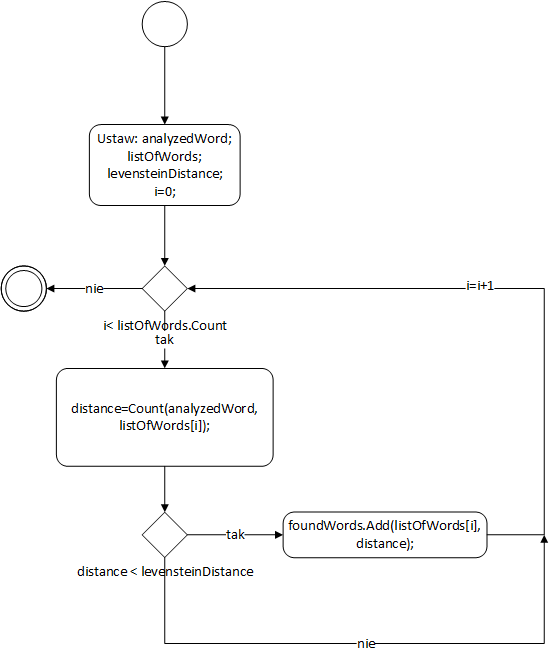
\includegraphics[width=0.6\linewidth]{rozdzial02/Levenstein1.png}
	\caption{Diagram dla działania algorytmu z wykorzystaniem odległości Levenshteina}
	\label{fig:Lev}
\end{figure}

\begin{figure} [H]
	\centering
	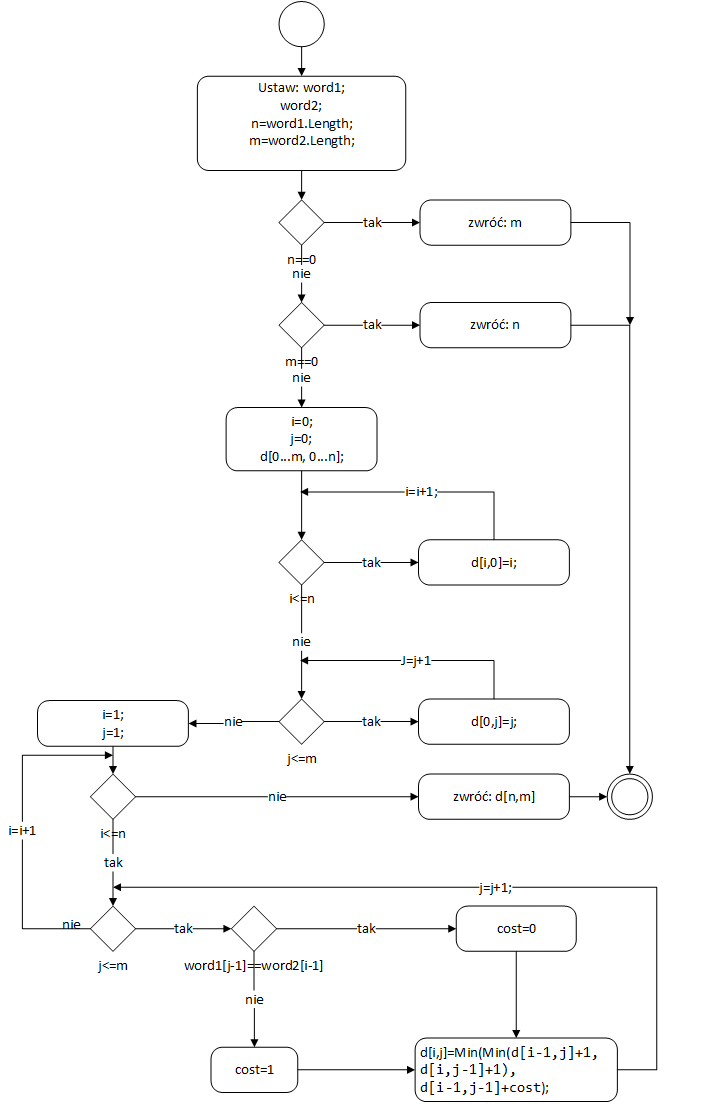
\includegraphics[width=1\linewidth]{rozdzial02/Levenstein-Count.png}
	\caption{Diagram obliczania odległości Levenshteina}
	\label{fig:Lev-Count}
\end{figure}


\section{LetterChanger}
\label{chap:Letter}
Ten algorytm do swojego działania potrzebuje listy najczęściej popełnianych błędów ortograficznych. Wybrane ciągi znaków i ich odpowiedniki ustawione zostały w liście \_letterPairs, co przedstawione zostało na listingu~\ref{lst:letter}. Są to według autorów projektu ciągi znaków, w których najczęściej popełniane zostają błędy ortograficzne. 

\lssetdef
\lstinputlisting[captionpos=b,caption={Lista par ciągów znakowych odpowiadająca najczęstszym błędom w języku polskim},label={lst:letter},basicstyle={\footnotesize\ttfamily}]{rozdzial02/letterPairs.txt}

Badany ciąg znaków, zostaje sprawdzony pod względem obecności ciągów znaków, z powyższej listy, z parametru Key. Następnie badany ciąg znaków zostaje przekształcany, poprzez zamienianie wszystkich "podejrzanych o błąd" fragmentów na ich zamienniki, czyli na ciągi znaków z parametru Value. Na przykład ciąg znaków ,,grzegrzółka'', pod wpływem zamian wynikających z pierwszego elementu listy \_letterPairs może przyjąć następujące trzy formy: ,,gżegrzółka'', ,,grzegżółka'' oraz ,,gżegżółka''. Wszystkie te trzy formy zostają wychwycone przez algorytm i zwrócone do programu w dalszym etapie. Przy okazji tego ciągu znaków, badane są również wszystkie ciągi znaków z uwzględnieniem zamiany ,,a'' na ,,ą'' oraz ,,e'' na ,,ę'', czyli m. in. powstają takie kombinacje jak ,,gżęgrzółką'', ,,grzegrzółką''.  Gdyby badany ciąg znaków tworzył ,,grzegrzulka'' to dodatkowo badane byłyby wszystkie kombinacje zamieniające ,,u'' na ,,ó'' oraz ,,l'' na ,,ł''. Algorytm ten powstał w celu łatwiejszego znajdywania tych kombinacji, których ilość podstawowych zamian na napisie, opisanych w poprzednim podrozdziale~\ref{chap:Lev}, może sugerować, że zostało wykonanych wiele operacji, a tak na prawdę został popełniony np. jeden błąd ortograficzny, dobrym przykładem jest tutaj zamiana ,,cz'' na ,,trz''. Również biorąc pod uwagę, że z powodów optymalizacyjnych, przy mierzeniu odległości Levenshteina, nie jest badany cały słownik, a jedynie najbardziej prawdopodobne jego fragmenty, ten algorytm doskonale wychwytuje pozostałe nieprawidłowości w badanym ciągu znaków. Schemat działania tego algorytmu został przedstawiony na diagramie z rysunku~\ref{fig:LetterChanger}. Algorytm ten znajduje więc dość dużo różnych ,,dziwnych'' kombinacji, jednak w dalszym etapie wszystkie te kombinacje podlegają sprawdzeniu, czy występują w słowniku i na tej podstawie określane jest czy zostaną podpowiedziane użytkownikowi czy też nie.

\begin{figure} [H]
	\centering
	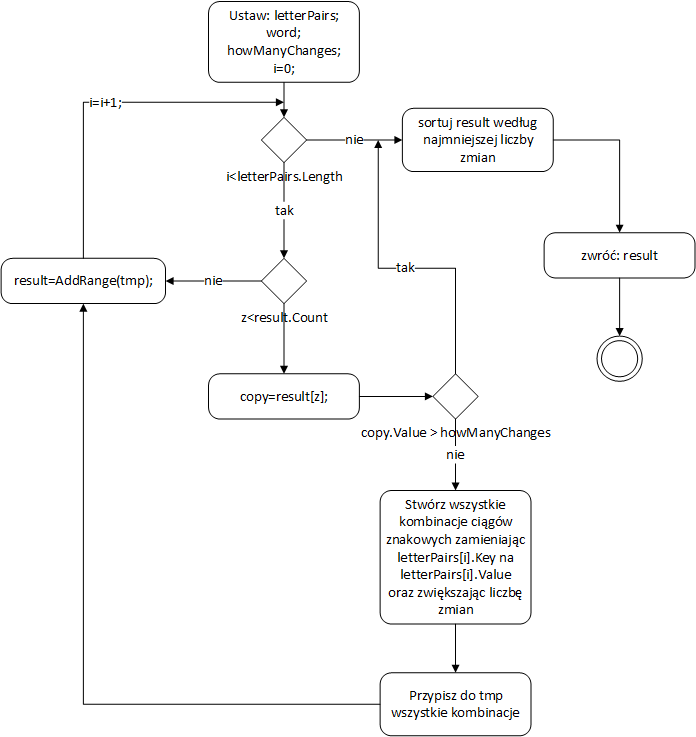
\includegraphics[width=1\linewidth]{rozdzial02/LetterChanger.png}
	\caption{Diagram zamieniania ciągów znaków odpowiadających najczęstszym błędom ortograficznym}
	\label{fig:LetterChanger}
\end{figure}

\section{SpaceAdder}
Algorytm ten powstał w celu wychwytywania, błędów, które na co dzień nie mają miejsca w piśmie ręcznym, jednak są powszechnym problemem w podczas opracowywania tekstów na komputerze. Mianowicie problem ten dotyczy braku wciśnięcia, bądź też reakcji komputera na wciśnięcie klawisza spacji. Algorytm ten bierze pod uwagę, że w jednym ciągu znakowym może wystąpić tylko jedno takie zdarzenie. Na przykład między innymi z ciągu znaków "idziekot" zostanie przekształcony do postaci "idzie kot", ale również do postaci "idzi ekot". Algorytm ten nie tworzy zbyt wielu kombinacji, jednak rozwiązuje dość często popełniany błąd w pisowni komputerowej. Dodatkowo w dalszym etapie działania programu kombinacje uzyskane z tego algorytmu podlegają też zamianom w oparciu o algorytm LetterChanger opisanym w podrozdziale~\ref{chap:Letter}, dzięki czemu również znajdywane są sugestie dla słów, w których popełniony został błąd ortograficzny oraz zabrakło spacji. Diagram UML, dla tego algorytmu został przedstawiony na grafice~\ref{fig:SpaceAdder}. 

\begin{figure} [H]
	\centering
	
\includegraphics[width=0.6\linewidth]{rozdzial02/SpaceSearcher.png}
	\caption{Diagram działania funkcji dodającej przerwy między wyrazami}
	\label{fig:SpaceAdder}
\end{figure}



